\documentclass[tikz,border=3pt]{standalone}
\usepackage[utf8]{inputenc}
\usepackage[T1]{fontenc}
\usepackage{lmodern}
\renewcommand{\familydefault}{\sfdefault}
\usepackage{sansmath}\sansmath
\usepackage{chemfig}
\usepackage{pgfplots}\pgfplotsset{compat=1.18,/pgf/number format/use comma,/pgf/number format/1000 sep={.}}
\usetikzlibrary{arrows.meta,calc,positioning,decorations.pathmorphing,patterns}
% paleta del sitio
\definecolor{nar}{HTML}{E8680C}\definecolor{narc}{HTML}{FFB35C}\definecolor{hielo}{HTML}{FFF3E8}
\definecolor{tinta}{HTML}{1D1D1F}\definecolor{gris}{HTML}{6E6E73}\definecolor{lila}{HTML}{7C5CF0}
\definecolor{azul}{HTML}{2F6FD6}\definecolor{menta}{HTML}{17A673}\definecolor{coral}{HTML}{E8342A}
\begin{document}
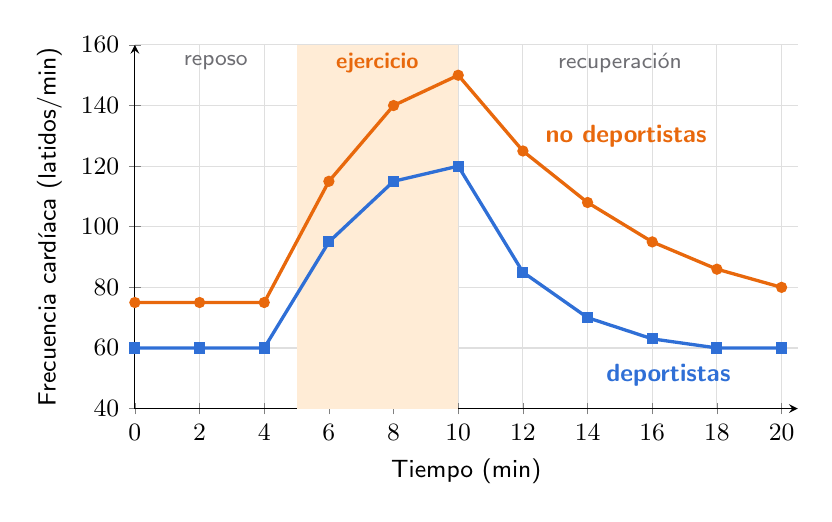
\begin{tikzpicture}[font=\small]
\begin{axis}[width=10cm,height=6.2cm,axis lines=left,xmin=0,xmax=20.5,ymin=40,ymax=160,xtick={0,2,...,20},ytick={40,60,...,160},
  grid=major,grid style={gray!25},xlabel={Tiempo (min)},ylabel={Frecuencia cardíaca (latidos/min)},clip=false]
\fill[narc!25] (axis cs:5,40) rectangle (axis cs:10,160);
\node[font=\footnotesize\bfseries,text=nar] at (axis cs:7.5,154) {ejercicio};
\node[font=\footnotesize,text=gris] at (axis cs:2.5,154) {reposo};
\node[font=\footnotesize,text=gris] at (axis cs:15,154) {recuperación};
\addplot[nar,very thick,mark=*,mark options={fill=nar,scale=0.7}] coordinates {(0,75)(2,75)(4,75)(6,115)(8,140)(10,150)(12,125)(14,108)(16,95)(18,86)(20,80)};
\addplot[azul,very thick,mark=square*,mark options={fill=azul,scale=0.7}] coordinates {(0,60)(2,60)(4,60)(6,95)(8,115)(10,120)(12,85)(14,70)(16,63)(18,60)(20,60)};
\node[nar,font=\small\bfseries,anchor=west] at (axis cs:12.4,130) {no deportistas};
\node[azul,font=\small\bfseries,anchor=north] at (axis cs:16.5,58) {deportistas};
\end{axis}
\end{tikzpicture}
\end{document}
